\begin{figure}[htbp]
\centering
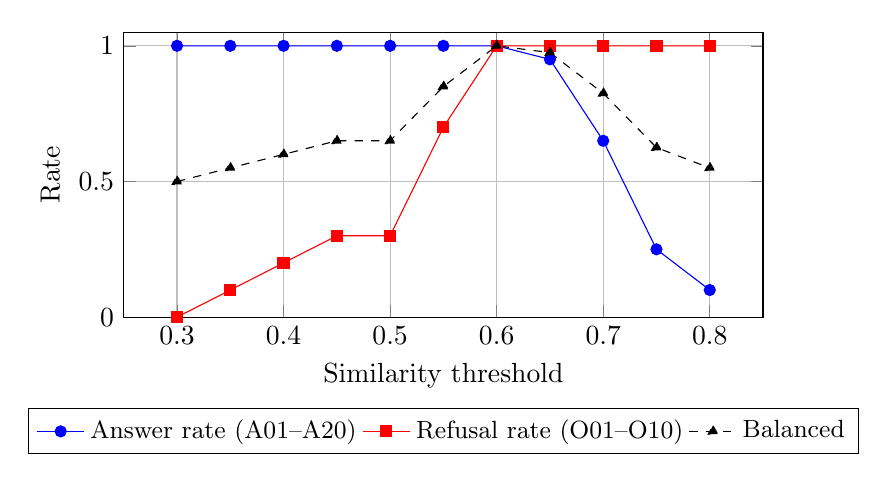
\begin{tikzpicture}
\begin{axis}[width=0.8\linewidth, height=5.2cm, xlabel={Similarity threshold}, ylabel={Rate}, ymin=0, ymax=1.05, grid=major, legend columns=3, legend style={at={(0.5,-0.32)}, anchor=north, font=\small}]
\addplot[blue, mark=*] coordinates {(0.3,1.0) (0.35,1.0) (0.4,1.0) (0.45,1.0) (0.5,1.0) (0.55,1.0) (0.6,1.0) (0.65,0.95) (0.7,0.65) (0.75,0.25) (0.8,0.1)};
\addlegendentry{Answer rate (A01--A20)}
\addplot[red, mark=square*] coordinates {(0.3,0.0) (0.35,0.1) (0.4,0.2) (0.45,0.3) (0.5,0.3) (0.55,0.7) (0.6,1.0) (0.65,1.0) (0.7,1.0) (0.75,1.0) (0.8,1.0)};
\addlegendentry{Refusal rate (O01--O10)}
\addplot[black, dashed, mark=triangle*] coordinates {(0.3,0.5) (0.35,0.55) (0.4,0.6) (0.45,0.65) (0.5,0.65) (0.55,0.85) (0.6,1.0) (0.65,0.975) (0.7,0.825) (0.75,0.625) (0.8,0.55)};
\addlegendentry{Balanced}
\end{axis}
\end{tikzpicture}
\caption{Answer rate, refusal rate and their mean (balanced) against the similarity threshold, on the original 30 questions (from \texttt{results/threshold\_sweep.csv}).}
\label{fig:sweep}
\end{figure}
